%%%%%%%%%%%%%%%%%%%%%%%
%%  Capítulo 4: Aplicación a estructras microstrip  %%
%%%%%%%%%%%%%%%%%%%%%%%

%%%%
\section{Introducción}

Como se describió en la sección \ref{subsec_antenas_microstrip}, las antenas \textit{microstrip} son utilizadas en un amplio rango de aplicaciones comerciales y militares, especialmente debido a que son livianas, de bajo perfil, suponen reducidos costos y resultan de fácil fabricación. Además, permiten diseños integrados con componentes activos, circuitos de microondas y elementos radiantes \cite{Yang:EBGAntennas}.

El tamaño de las antenas está íntimamente ligado a la longitud de onda de trabajo, que se relaciona a la frecuencia y permitividad eléctrica del sustrato utilizado, como queda explícito en la ecuación \ref{eq:frecRes-modosSup-microstripAntenna}. Al mismo tiempo, dado que en general son antenas resonantes, presentan un alto Q, lo que afecta a su ancho de banda.

En muchos casos es necesario disminuir el tamaño de los elementos \textit{microstrip}, lo que se puede lograr mediante cortocircuitos y líneas \textit{microstrip} de formas complejas. Otro método, más sencillo, consiste en aumentar el valor de la permitividad eléctrica del sustrato. Sin embargo, como ya se explicó antes, y como se puede observar en la figura \ref{fig:zstm-permit-diel}, el aumento de este parámetro aumenta el valor de la impedancia inductiva de la superficie, permitiendo el desarrollo de ondas de superficie.

Por otro lado, el uso de dieléctricos de constante alta genera un ancho de banda aún menor (un mayor Q) y aún más baja eficiencia de radiación. Estos efectos suelen mitigarse con el aumento del ancho del sustrato, que, en contrapartida, genera condiciones propicias para la propagación de ondas de superficie en modo TM, debido a que, como se indica en la ecuación \ref{eq:campo-magnetico-interior-diel-TM} y se esquematiza en la figura \ref{fig:soluciones-TM-tan-implicita-zoom}, se permiten una mayor cantidad de modos de propagación en el eje $x$ (vertical). Por otro lado, un análisis de la impedancia de superficie indica que el comportamiento inductivo aumenta con el ancho del sustrato (ecuación \ref{eq:impedancia-superficie-tm-teorica} y figura \ref{fig:Zstm-parametros}), lo que también es signo de una configuración que soporta ondas de superficie con facilidad.

Las ondas de superficie, además, extraen potencia que no se convierte en radiación y, facilitan el acoplamiento entre elementos. Además, cuando inciden sobre discontinuidades, generan lóbulos secundarios que degradan el patrón de radiación y las características de polarización \cite{Balanis:Theory}.

Entre las distintas técnicas que han surgido para la disminución de la presencia de ondas de superficie en el sustrato que soporta a las antenas \textit{microstrip}, entre las que destacan las relativas a disminuir la altura del sustrato en los bordes de la antena (figura \ref{fig:escalon-sustrato}), en los últimos años ha cobrado especial interés el uso de sustratos con banda prohibida electromagnética, debido a que no requieren un cambio en la tecnología de fabricación. Los mismos pueden aplicarse justo debajo de la antena (generando estructuras planares que reemplazan al plano de tierra, conocidas como DGS, que ofrecen como contrapartida un diagrama de radiación con mayores lóbulos laterales), o alrededor de la misma (\cite{Marcela:Tesis}, figura \ref{fig:sustrato-antena-ebg}). Ambas soluciones, debido a la naturaleza resonante de la antena, que genera que las frecuencias en juego estén distribuidas en un ancho de banda acotado, tienen como consecuencia una disminución del acoplamiento mutuo con elementos circuitales cercanos a la antena (en particular, otras antenas que podrían estar formando parte de un arreglo de radiadores). Esto es así porque, si las estructuras que rodean al elemento radiante tienen una banda prohibida para las frecuencias de trabajo, las mismas no podrán propagarse por el sustrato.


\begin{figure}[H]
	\centering 
	\subfigure[Antena rodeada por una estructura EBG.]{
		\label{fig:sustrato-antena-ebg}
		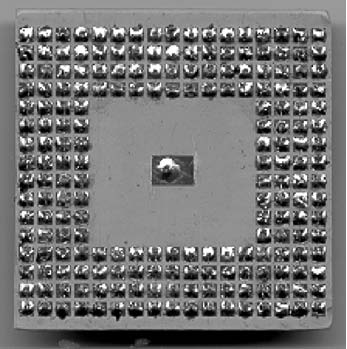
\includegraphics[width=0.35\textwidth]{Aplicacion/foto-ebg-alrededor-antena.pdf}}
	\hspace{30pt}
	\subfigure[Antena rodeada por un escalón de sustrato,]{
		\label{fig:escalon-sustrato}
		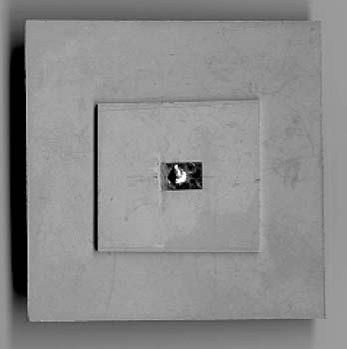
\includegraphics[width=0.45\textwidth]{Aplicacion/foto-escalon-alrededor-antena.pdf}}
	\caption{Fotos de diseños de antenas parches con limitadores a la propagación de onda de superficie \cite{Yang:EBGAntennas}}
	\label{fig:limitadores-ondas-superficie-yang}
\end{figure}

Las primeras estructuras EBG utilizadas con estos fines consistían en arreglos de agujeros cilíndricos en el sustrato que, debido a la periodicidad que presentaban para las ondas de superficie, daban lugar a un comportamiento de filtro, presentando una banda prohibida. La dificultad para la fabricación de este tipo de sustratos dio lugar a la búsqueda de estructuras de banda prohibida de mayor facilidad de uso. En 1999, Sievenpiper presentó, en sus tesis doctoral \cite{Sievenpiper:Thesis}, una estructura que denominó HIS (\textit{High Impedance Surface}, superficie de alta impedancia), que además de cumplir con las características de un conductor magnético para un rango de frecuencias \cite{Sievenpiper:HIESForbiddenBand} y de ser de fácil fabricación con tecnología \textit{microstrip}, poseía también una banda prohibida electromagnética para las ondas de superficie \cite{Marcela:Tesis}. Esta estructura, consistente en parches metálicos dispuestos sobre un sustrato, y unidos al plano de tierra, ubicado en la cara opuesta del mismo, a través de vías metálicas, redujo ampliamente los costos y la dificultad de fabricación. Pocos años más tarde, debido a que en algunos casos el uso de vías retrasa la fabricación de circuitos \textit{microstrip}, surgieron estructuras de banda prohibida uniplanares, con características similares, aunque con anchos de banda prohibida más reducidos.

Para el presente trabajo, estas estructuras se ubicarán entre dos antenas microstrip, alineadas según distintos criterios, a fin de comparar el diagrama de radiación y el acoplamiento mutuo con el que se logra con el mismo arreglo radiante, pero sin el uso de EBG entre ellas.

% Coccioli, Yang, Itoh, intro historica.
\section{Técnicas de aumento del ancho de banda para el análisis}
\label{sec_aumento_bw}
%%%%
\lipsum
% Rahmat. Pagina 127, libro. Efecto de algunos parámetros.}
% Paper Kumar, Gupta, Nonradiating
% Notar que paper de Assimonis, Yioultsis no usa esto. MAL.
%%%%
\section{Diseño de la antena microstrip}
\label{sec_disenio_microstrip}
%%%%
\lipsum
% Pablito. Cst.
% Condiciones de borde: LIbroSinNombre, pagina 398.
%%%%
\section{Elección del metamaterial}
\label{sec_eleccion}
%%%%
\lipsum
% Cantidad de celdas minima: Bouali, Aguili, impreso.
% Pedir que bw del metamaterial sera mayor al de la antena
% Mirar el analisis de Coccioli, Yang, Itoh, pag 2126
% ¿criterio para la distancia? IMPORTANTE!!!!!
%%%%
\section{Estudio del efecto sobre el acoplamiento mutuo}
\label{sec_estudio_acoplam_mutuo}
%%%%
\lipsum
% Ondas de superficie se proparagan por plano E? Pagina 132. Rahmat, lbro,.
% Pagina 138. Rahmat.
% Efecto según la orientacion de parches. ABidin, Tesis, Pagina 37.
% Algo se puede ver en Assimonis, Yioultsis, Antonopoulos
%%%%
\section{Estudio del efecto de la distancia sobre el ancho de banda}
\label{sec_efecto_distancia}
%%%%
\lipsum
%Coccioli, Yang, Itoh, pag 2127
% Iluz, Shavit, pag 1448

% Ver que overall las conclusiones son similares a Islam,Alam.
